% !TeX spellcheck = en_GB
\documentclass[10pt,letterpaper,oneside]{article}
\usepackage{fontspec}
\usepackage{arev}
\usepackage[utf8]{inputenc}
\usepackage[T1]{fontenc}
\usepackage{amsmath}
\usepackage{amsfonts}
\usepackage{amssymb}
\usepackage{graphicx}
\usepackage{csquotes}
\usepackage{booktabs}
\usepackage{multicol}
\usepackage{enumerate}
\usepackage{microtype}
\usepackage[labelfont=bf,font={small}]{caption}
\usepackage{hyperref}
\usepackage{booktabs}
\usepackage{subcaption}
\usepackage{fancyhdr}
\usepackage{calc}
\usepackage[svgnames]{xcolor}
\usepackage{cleveref}

\newfontfamily\symbolfont{Symbola}
\usepackage[left=1in,right=1in,top=1in,bottom=1in,marginparwidth=0.25in]{geometry}

\usepackage[sorting=none]{biblatex}
\addbibresource{../bibliography.bib}

\author{Andreas Stöckel\\[0.5cm]Based on lecture notes by\\Chris Eliasmith and Terrence~C.~Stewart}

\fancyhf{}
\fancyhead[L]{SYDE 556/750 Lecture Notes}
\fancyhead[R]{Andreas Stöckel}
\fancyfoot[C]{\thepage}
\pagestyle{fancy}

\setlength{\parindent}{0em}
\setlength{\parskip}{0.5em}
\renewcommand{\baselinestretch}{1.25}
\renewcommand{\vec}[1]{{\mathbf{\mathrm{#1}}}}
\newcommand{\mat}[1]{{\mathbf{\mathrm{#1}}}}

\newcommand{\MakeTitle}[1]{
\maketitle
\begin{center}
	\includegraphics[width=0.5\textwidth]{../assets/uwlogo.pdf}\\[1cm]
	{#1}\
\end{center}

\vfill

\thispagestyle{empty}
\setcounter{page}{0}
\newpage

\pagenumbering{roman}
\tableofcontents
\newpage

\setcounter{page}{0}
\pagenumbering{arabic}}

\reversemarginpar

\newcommand{\ColorBox}[3]{{\par\hspace{0pt}\marginpar{\huge\raisebox{-1ex}{\symbolfont{#1}}}\ignorespaces\fboxsep=0.5cm\colorbox{#2}{\begin{minipage}[t]{\columnwidth-1cm}{#3}\end{minipage}}}}

\newcommand{\Note}[1]{\ColorBox{📌}{WhiteSmoke}{\textbf{Note:} #1}}
\newcommand{\Example}[1]{\ColorBox{💡}{WhiteSmoke}{\textbf{Example:} #1}}


\date{January 9, 2020}
\title{SYDE 556/750 \\ Simulating Neurobiological Systems \\ Lecture 2: Neurons}


\begin{document}

\MakeTitle{\textbf{Accompanying Readings: Chapter 2.1 and Chapter 4.1 of Neural Engineering}}

\section{Overview}

As we have discussed in the last lecture, we consider neurons to be the fundamental computational element in the nervous system. (Most) neurons communicate by generating action potentials (or spikes) that are sent to and received by post-synaptic neurons.

An important part of understanding nervous systems is thus to understand the \enquote{code} that is being exchanged between neurons. Unfortunately, there is no scientific consensus about what exactly \enquote{the neural code is}. What we do have, are very detailed models of how individual neurons generate spikes. Thus, we will approach the problem of neural representation in two stages. First, in this lecture, we will have a look at single neurons and try to get an understanding of how neurons generate action potentials. Second, in the next two lectures, we will use information theory to think about what a potential neural representation could be.

\section{Spiking Neurons}

\Note{We're going to have a slightly closer look at biologically detailed spiking neuron models towards the end of the class. For now, we're skimming over the details a little. Feel free to have a look at \cite{kandel2012principles} if you want to learn more about basic neurobiology.}

\begin{figure}[t]
	\centering
	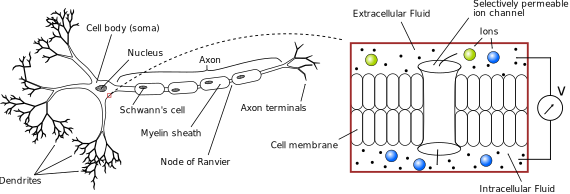
\includegraphics{media/neuron_sketch_membrane.pdf}
	\caption{Illustration showing a text-book neuron, as well as a schematic cross-section through the cell membrane. Left part of the illustration from \cite{stoeckel2015design}, adapted from \cite{kandel2012principles}}
	\label{fig:neuron_sketch_membrane}
\end{figure}

Neurons are cells that specialise in the integration and transfer of electrical signals. Cells are generally separated from the environment by a thick, impermeable \enquote{barrier}, the \emph{cell membrane}, consisting of a bi-layer of lipid molecules. The cell membrane establishes an \enquote{intra-cellular} space that is isolated from the \enquote{extra-cellular} space. Both spaces are filled with a watery liquid, the \emph{intra-cellular fluid} and \emph{extra-cellular fluid}, respectively (\cref{fig:neuron_sketch_membrane}).

\subsection{Qualitative neural behaviour}

\begin{figure}
	\centering%
	\begin{subfigure}{0.5\textwidth}%
		\centering
		\includegraphics{media/hh_neuron_sub_threshold.pdf}%
		\caption{Sub-threshold neuron}%
		\label{fig:hh_neuron_sub_threshold}
	\end{subfigure}%
	\begin{subfigure}{0.5\textwidth}%
		\centering
		\includegraphics{media/hh_neuron_super_threshold.pdf}%
		\caption{Super-threshold neuron}%
		\label{fig:hh_neuron_super_threshold}
	\end{subfigure}%
	\caption{Computer simulation of a Hodgkin Huxley model neuron \cite{hodgkin1952quantitative,traub1991neuronal}. The blue line corresponds to the membrane potential $v$, the dashed line to the current $J$ that is being injected into the neuron.}
\end{figure}

When we stick a sharp electrode into a neuron (akin to the \enquote{single electrode recording}), we can measure a difference in electrical potential, i.e.~a voltage $v$ between the inside and the outside of the cell (\cref{fig:neuron_sketch_membrane}). We call this initial voltage the \emph{resting potential} $E_\mathrm{L}$.\footnote{The weird symbol \enquote{$E_\mathrm{L}$} stems the more precise name of this potential, the \enquote{\textbf{L}eak channel \textbf{E}quilibrium potential}.}

Instead of just measuring this potential we may also inject an external current into the neuron by hooking it up to a current source (i.e.~a power supply that regulates current instead of voltage). When doing this, we find four things:
\begin{enumerate}
	\item The cell acts like a \emph{capacitor}, i.e., the voltage increases while we're injecting a current (\cref{fig:hh_neuron_sub_threshold}).
	\item The capacitor is \emph{leaky}. As soon as we stop injecting a current, the voltage collapses back to the resting potential $v_\mathrm{rest}$ injecting a current (\cref{fig:hh_neuron_sub_threshold}).
	\item As soon as the voltage surpasses a certain value, the \emph{threshold potential} $v_\mathrm{th}$, the cell will generate a spike.
	\item Shortly after the spike has been produced, the voltage drops below the resting potential. During this period, the \emph{refractory period} of length $\tau_\mathrm{ref}$ we cannot get the neuron to spike again, even if we apply large input current $J$.
\end{enumerate}

\Note{Imporatantly, neurons in biology are \emph{dynamical systems}, i.e., they possess a behaviour that evolves over time. \emph{Artificial neurons} (see below) are time-independent. They are mathematical functions that take an input and \enquote{immediately} map it onto an output.}

\subsection{The Leaky Integrate and Fire Neuron}

We can qualitatively summarize this behaviour in a very simple model, the so called \enquote{Leaky Integrate and Fire} neuron model. This model was first proposed by the French scientist Louis Lapicque in 1907 \cite{lapicque1907recherches,abbott1999lapicque}.

\paragraph{Sub-threshold behaviour}
First, we have the \emph{sub-threshold} behaviour, a so called leaky integrator.
\begin{align}
	\begin{aligned}
		\frac{\mathrm{d}}{\mathrm{d}t} v(t) &= \frac{1}{C_\mathrm{m}} \big(g_\mathrm{L} (E_\mathrm{L} - v(t))
			+ J
		\big) \,, \quad \text{if } v(t) < v_\mathrm{th}\,.
	\end{aligned}
	\label{eqn:sub-threshold}
\end{align}
This differential equation corresponds to a capacitor with capacity $C_\mathrm{m}$ that is charged with a current $J$ and that slowly discharges to a potential $v_\mathrm{reset}$ over a resistor with conductance (the inverse of the resistance) $g_\mathrm{L} = \frac{1}{R}$ (the \emph{leak conductance}).

\paragraph{Super-threshold behaviour}
Second, we have the \emph{super-threshold behaviour}, the spike production and refractory period. Assume $v(t) = v_\mathrm{th}$ at $t = t_\mathrm{th}$. Then
\begin{align}
	\begin{aligned}
		v(t) &= \delta(t - t_\mathrm{th}) \,, &\text{if } t &= t_\mathrm{th} \,,\\
		v(t) &= v_\mathrm{reset} \,, &\text{if } t &> t_\mathrm{th} \text{ and } t \geq t_\mathrm{th} + \tau_\mathrm{ref} \,,
	\end{aligned}
	\label{eqn:super-threshold}
\end{align}
where $\delta(t)$ is the Dirac delta function, i.e., the function defined as
\begin{align*}
	\delta(t) &= \begin{cases} \infty & \text{if } t = 0 \, \\ 0 & \text{if } t \neq 0 \,, \end{cases}  \quad \text{ and } \quad \int_{-\infty}^\infty \delta(t)\,\mathrm{d}t = 1 \,.
\end{align*}

\paragraph{Normalized equations}
For our modelling purposes, we don't really care about the exact values of $v_\mathrm{th}$, $v_\mathrm{reset}$ and $E_\mathrm{L}$. We can just normalise these voltages, i.e., assume that $v_\mathrm{th} = 1$, and $v_\mathrm{reset} = E_\mathrm{L} = 0$.

We can rewrite \cref{eqn:sub-threshold,eqn:super-threshold} as
\begin{align}
	\begin{aligned}
		\frac{\mathrm{d}}{\mathrm{d}t} v(t) &= -\frac{1}{\tau_\mathrm{RC}} \big( v(t) - RJ \big)
		\big) \,, \quad &\text{if } v(t) &< v_\mathrm{th}\,. \\
		v(t) &= \delta(t - t_\mathrm{th}) \,, &\text{if } t &= t_\mathrm{th} \,,\\
v(t) &= 0 \,, &\text{if } t &> t_\mathrm{th} \text{ and } t \geq t_\mathrm{th} + \tau_\mathrm{ref} \,,
	\end{aligned}
	\label{eqn:sub-threshold-normalised}
\end{align}
where, $\tau_\mathrm{RC} = C_\mathrm{m} R$ and $R = \frac{1}{g_\mathrm{L}}$.

\subsection{Characterizing the LIF Neuron}

\begin{figure}[t]
	\begin{subfigure}{\textwidth}
		\centering
		\includegraphics{media/hh_neuron_ramp.pdf}
		\caption{Hodgkin-Huxley model neuron}
	\end{subfigure}
	\begin{subfigure}{\textwidth}
		\centering
		\includegraphics{media/lif_neuron_ramp.pdf}
		\caption{Normalized Leaky Integrate-and-Fire neuron}
	\end{subfigure}
	\caption{Effects of a current ramp on an Hodgkin-Huxley type model neuron and a (normalized) LIF neuron. As above, the blue line is the membrane potential, the dashed line is the input current.}
\end{figure}

\section{Artificial Neurons}

%Embedded into the cell membrane are special proteins that act as gateways for matter that flows into or out of the cell. These proteins may either actively transport matter, or passively act as a filter that only lets certain kinds of matter through (\cref{fig:neuron_sketch_membrane}).

%\subsection{Reducing Neurons to a Single Point}

%\begin{figure}[t]
%	\centering%
%	\begin{subfigure}{0.5\textwidth}%
%		\centering%
%		\includegraphics{media/neuron_channel_a.pdf}%
%		\caption{Neuron in resting state}%
%		\label{fig:neuron_channel_a}
%	\end{subfigure}%
%	\begin{subfigure}{0.5\textwidth}%
%		\centering%
%		\includegraphics{media/neuron_channel_b.pdf}%
%		\caption{After adding a selectively permeable ion channel}%
%		\label{fig:neuron_channel_b}
%	\end{subfigure}
%	\caption{Effects of a semipereable ion channel on the neural potential. \textbf{(a)} The neuron is in a resting state, and the intra- and extra-cellular fluid is electrectically neutral. \textbf{(b)} Once we add a semi-permeable ion channel, a new equilibrium state will be created by countering osmotic and electrical forces. From \cite{stoeckel2015design}, adapted from \cite{reichert2000neurobiologie}.}
%\end{figure}

%The intra- and extra-cellular fluids contain electrically charged particles, mostly ions and some complex electrically charged molecules. To simplify things a little, let's assume that the fluid on the in- and outside of the cell is homogeneous, i.e.~has the same properties everywhere. Correspondingly, we can collapse the entire elaborately shaped neuron into a small sphere -- the only thing that matters when we measure ion concentrations or electrical potentials is whether we're on the inside or the outside of the cell.

%When we measure ion concentrations of the intra-cellular fluid and the extra-cellular fluid, we find that both fluids are electrically neutral, yet contain different concentrations of ions.\footnote{Special \enquote{ion pump} proteins in the cell membrane ensure over long periods of time that this mixture approximately stays the same.} The cells being electrically \emph{neutral} means, that there is nothing interesting  (\cref{fig:neuron_channel_a}).


%\subsection{Spike Production: The Hodgkin Huxley Neuron Model}

%\section{The Leaky Integrate and Fire Neuron Model}

%\section{Artifical Neurons}


\printbibliography

\end{document}